\chapter{Data Sets and Experimental Design}
\label{Chapter data sets}
In order to address our research questions, this thesis considered a group of data sets from the UCR data archive \cite{UCRArchive2018} and the UEA data archive \cite{bagnall2018uea}.
This Chapter will describe the data sets that were used to conduct our experiments and their general properties.
Then we will describe our experimental setup.

\section{UCR/UEA Archives}
\label{DataArchives}
The University of California Riverside (UCR) and the University of East Anglia (UEA) data archives have been used as references in literature for many experiments on time series problems \cite{abanda2019review,fawaz2020inceptiontime,bagnall2017great,yazdanbakhsh2019multivariate,ruiz2020great,fawaz2019deepreview}
and specially for benchmarking the performance of algorithms.

\subsection{UCR Archive}
\label{UCR}
The UCR archive previously had 85 univariate data sets, but in 2018 it was expanded to reach 128 data sets.
Despite sharing the property of being univariate, the data sets cover a variety of values for other aspects like;
training data size [16, 8926]; testing data size [20, 16800]; number of classes [2, 60]; length of time series [15, 2844] and for some data sets length of instances vary within the data set;
and the nature of the data being collected. The archive offers a single predefined train/test split for each of the data sets to facilitate reproducability of results.
Finally, the data is z-normalized; to remove offset and scaling. Z-normalization is the transformation of the data to have a mean of zero and one unit of standard deviation.

\subsection{UEA Archive}
\label{UEA}
The other archive we used is the UEA archive for multivariate data sets. Like the UCR archive, it was developed and expanded over time.
It started as a small archive of 12 data sets collected by Mustafa Baydogan,
then later on, in 2018, was expanded to reach 30 data sets as a collaboration between researchers of UEA and UCR. The data sets vary in their characteristics;
training data size [12, 30000]; testing data size [15, 20000]; number of classes [2, 39]; length of time series [8, 17984]; number of dimensions [2, 1345] and six different groups based on their application area.
The archive was processed so that the data instances have equal lengths, instances of missing data points were excluded and a single predefined train/test split is provided.

\subsection{Used Data Sets}
\label{used data sets}
For the scope of our experiment, a total of 77 data sets were selected from both archives to be used within the framework.
We have based our selection criteria for data sets on:
\begin{itemize}
    \item The data belongs to a real time series structure behind it and not converted from another data format.
    \item All instances in the data sets has the same length of time series.
    \item The data sets should not contain any missing values.
\end{itemize}
Based on the previously mentioned criteria, we excluded data sets that belonged to either of the types; Simulated, Image or Motion type; to comply with our first selection criteria.
For the other two criteria; we avoided any further preprocessing than what is offered by the data archives.
As mentioned before, the univariate data sets from the UCR are already Z-normalized.
Z-normalization is a common and recommended practice for time series data as it has shown to have a positive impact on the performance of classifiers \cite{bagnall2017great,fawaz2019deepreview}
This form of preprocessing is not T for the multivariate data sets from the UEA archive.

We excluded data sets with missing data and avoided filling these missing values; as we believe that data imputation is a whole another topic.
We also avoided any interpolation of data. A technique which has been previously used in \cite{ratanamahatana2005three, fawaz2019deepreview} to make all instances of the data set of the same length as the longest instance.
Our goal in this experiment is to focus on comparing the performance of the classifiers in our proposed context based while ensuring, as much as possible, that the main contributing factor is the technique behind the classifiers.
This doesn't mean that preprocessing of time series data is of a less importance, but we simply excluded it because we believe that it doesn't fit into our current scope.

The remaining collection of data sets still represented a wide variety in terms of data criteria.
We present the statistics about the remaining data sets all together in figure \ref{fig:DatasetsMetadata}.
Since the smallest data set (StandWalkJump) and the largest data set (InsectWingbeat) are the same as the UEA archive; training and testing data sizes are the same as previously mentioned ranges in the original archive, [12, 30000] and [15, 20000] respectively.
The data sets covers from binary classification problems up to problems with 52 classes, the range [2, 52].
The range of the time series length is [24, 3000], with Chinatown being the shortest and MotorImagery the longest data set.
For the 22 multivariate data sets, the number of dimensions still covered the whole range [2, 1345] like the UEA archive.
Finally after our exclusion criteria, the remaining 14 problem types are AUDIO, DEVICE, ECG, EEG, EOG, EPG, HAR, HEMO, MISC, OTHER, SENSOR, SOUND, SPECTRO and Traffic.

\begin{figure}
    \captionsetup{justification=raggedright}
    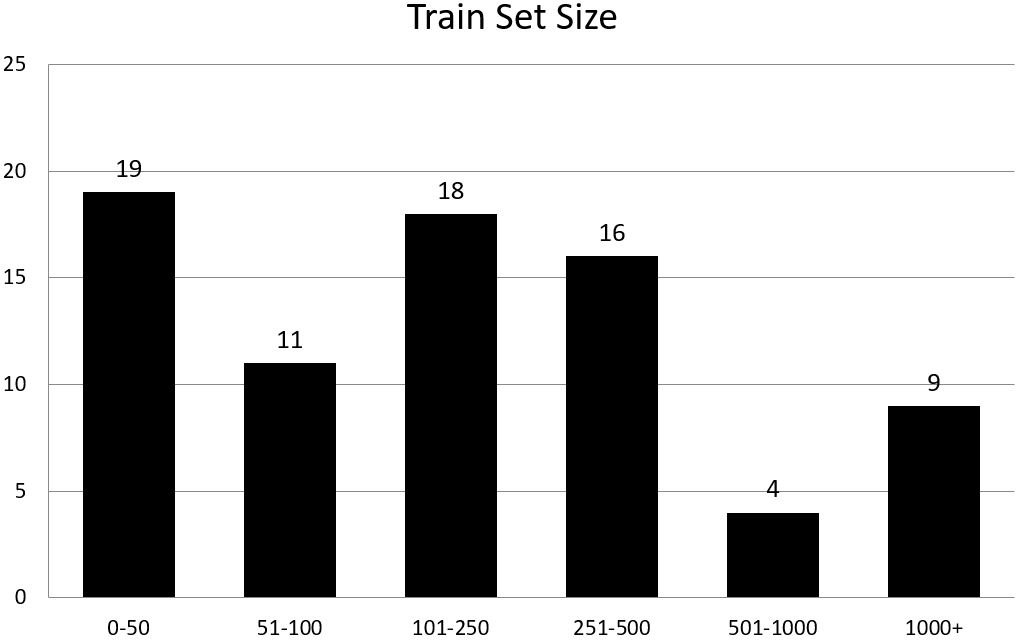
\includegraphics[width=0.49\textwidth,keepaspectratio]{Train_size_hist.JPG}
    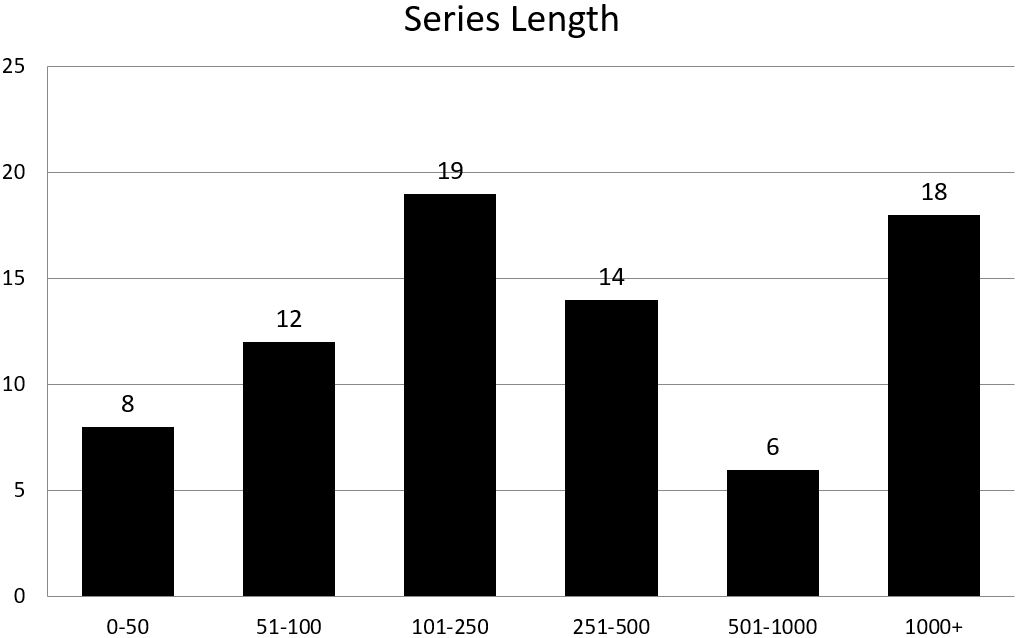
\includegraphics[width=0.49\textwidth,keepaspectratio]{Length_hist.JPG}
    \\[\smallskipamount]
    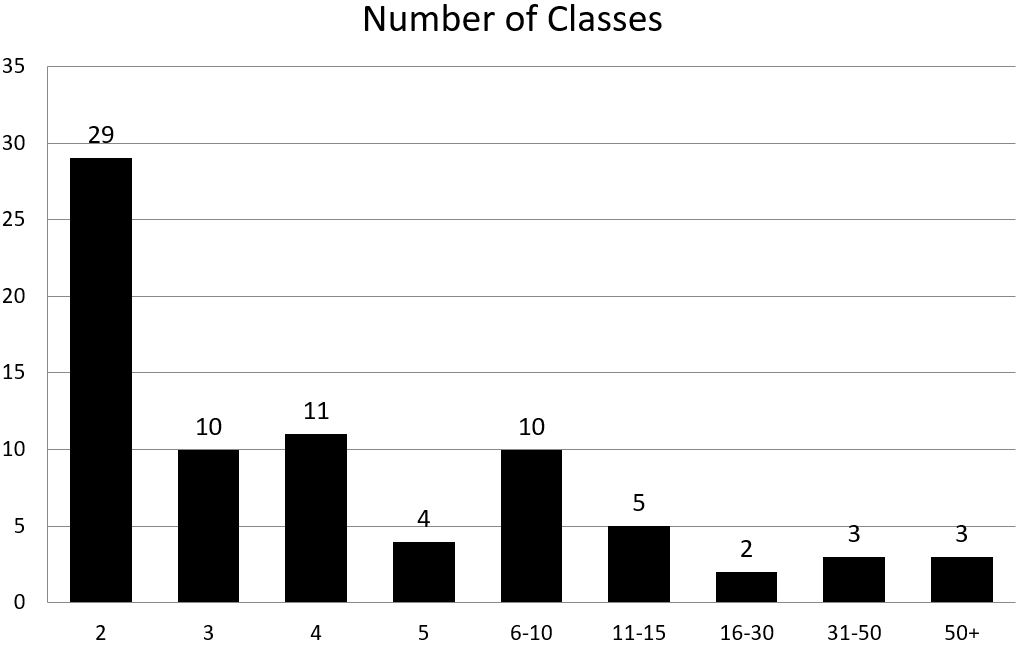
\includegraphics[width=0.49\textwidth,keepaspectratio]{Classes_hist.JPG}
    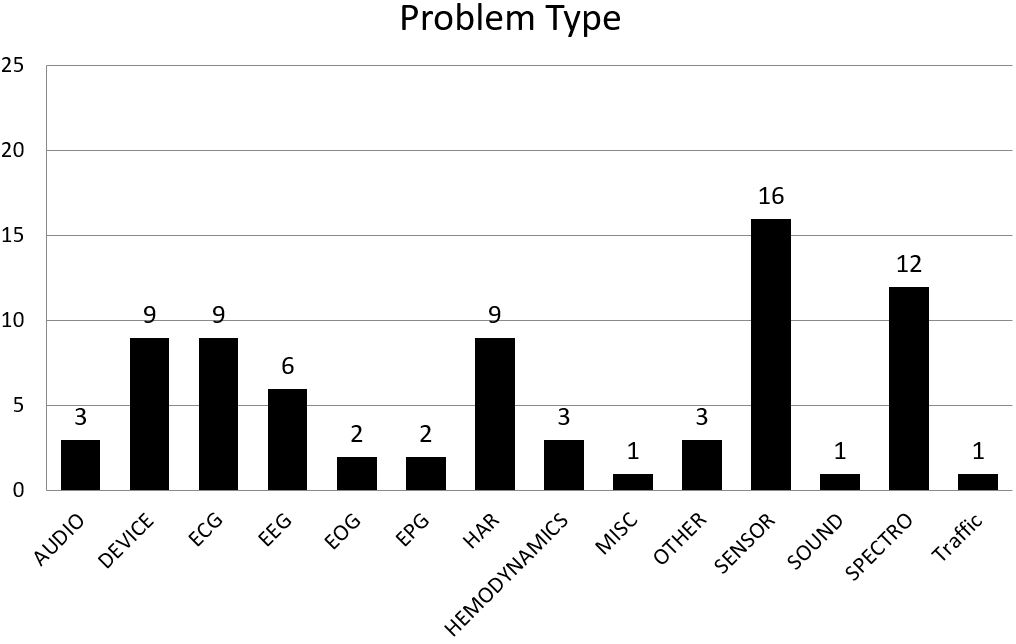
\includegraphics[width=0.49\textwidth,keepaspectratio]{Problem_hist.JPG}
    \caption{Metadata of the used data sets}
    \label{fig:DatasetsMetadata}
\end{figure}

Although the data sets that we used covered a variety of properties, but within some properties there were huge imbalances in the distribution of values.
Within grouping by training data set size, the group of data sets with sizes [501, 1000] was the smallest, with only 4 data sets which is less than half of the next smallest group.
Grouping by series length was the best, among the different groupings, in terms of imbalance. Data sets of lengths [501, 1000] were the smallest group with a count of 6 compared to the largest group, length [101, 250], of 19 data sets.
Number of classes was highly imbalanced; the binary classification group contained 29 data sets, which was more than double the second largest group [6, 10] of 10 data sets.
This is expected because all the data sets from the UCR archive fall into the same bin, while the multivariate data sets, which are already less in number, are distributed among multiple bins.
Finally, there was an over representation of type SENSOR than any other type with a total of 16 data sets.
While multiple other groups were represented by very few data sets like MISC, SOUND and TRAFFIC which only had 1 data set; or like EOG and EPG which had 2 data sets.


Since the final goal of our work is to learn a recommender which will be able to suggest the best performing classifier to unseen data sets based on their properties.
It is important to include all necessary and useful metadata about the data sets, which will help the recommender correctly give its recommendations.
Imblanced data sets can easily produce misleading results in terms of performance, specially if using a simple performance metrics like accuracy.
In cases of extreme imbalance, one can attain very high accuracy scores, simply by always predicting the majority class.
Handling the data imbalance is a two fold solution.
The first step to help learn about the skewness is to have a definition for imbalance. Then based on this definition flag the data sets as either having balanced classes or not.
The second step is to use a suitable performance metric which can give actual performance results and not be mislead by the imbalance.

We discuss the first step here as it is a feature of the data set, the other step we consider in the design of our experiments in section \ref{SectionExperiment}.
To be able to inform our recommender about the skewness property of a data set, we create a new feature, in addition to the previously discussed ones ; to indicate whether a data set is balanced in terms of class distribution or skewed.
We define a data set to be skewed if there exists a class in this data set which is, at least, as twice as likely as any other class.

To better exaplain how this property works, consider the two data sets; $DS_{1}$ and $DS_{2}$ each of which contains 5 classes.
$DS_{1}$ has a class distribution: $P(C_{1})$ =20\%, $P(C_{2})$ = 15\%, $P(C_{3})$ = 15\%, $P(C_{4})$ = 25\% and $P(C_{5})$ = 25\%.
While $DS_{2}$ has a class distribution: $P(C_{1})$ = 20\%, $P(C_{2})$ = 15\%, $P(C_{3})$ = 15\%, $P(C_{4})$ = 30\% and $P(C_{5})$ = 20\%.
In this case we would flag $DS_{1}$ as a balanced data set; because there is no prior class probability which is double any other.
On the other hand, $DS_{2}$ would be flaged as skewed/imbalanced because class $C_{4}$ has a probability of 30\% which is double the value
of $C_{2}$ and $C_{3}$. We denote this feature with the parameter $Balanced$, which is a boolean flag.

\begin{landscape}
    \begin{longtable}{|*{8}l|}
    %\begin{longtable}{\textwidth}{|c|c|c|c|c|c|c|c|}
        \hline
        \textbf{Dataset} & \textbf{Train Size} & \textbf{Test Size} & \textbf{Length} & \textbf{\#Classes} & \textbf{Type} & \textbf{\#Dim} & \textbf{Balanced} \\ [0.5ex]
        \hline
        \endfirsthead % <-- This denotes the end of the header, which will be shown on the first page only
        \hline
        \textbf{Dataset} & \textbf{Train Size} & \textbf{Test Size} & \textbf{Length} & \textbf{\#Classes} & \textbf{Type} & \textbf{\#Dim} & \textbf{Balanced} \\ [0.5ex]
        \hline
        \endhead % <-- Everything between \endfirsthead and \endhead will be shown as a header on every page
        ACSF1 & 100 & 100 & 1460 & 10 & DEVICE & 1 & T \\
        \hline
        AtrialFibrillation & 15 & 15 & 640 & 3 & ECG & 2 & T \\
        \hline
        BasicMotions & 40 & 40 & 100 & 4 & HAR & 6 & T \\
        \hline
        Beef & 30 & 30 & 470 & 5 & SPECTRO & 1 & T \\
        \hline
        Car & 60 & 60 & 577 & 4 & SENSOR & 1 & T \\
        \hline
        Chinatown & 20 & 345 & 24 & 2 & Traffic & 1 & T \\
        \hline
        CinCECGTorso & 40 & 1380 & 1639 & 4 & ECG & 1 & F \\
        \hline
        Coffee & 28 & 28 & 286 & 2 & SPECTRO & 1 & T \\
        \hline
        Computers & 250 & 250 & 720 & 2 & DEVICE & 1 & T \\
        \hline
        Cricket & 108 & 72 & 1197 & 12 & HAR & 6 & T \\
        \hline
        DuckDuckGeese & 60 & 40 & 270 & 5 & AUDIO & 1345 & T \\
        \hline
        Earthquakes & 322 & 139 & 512 & 2 & SENSOR & 1 & F \\
        \hline
        ECG200 & 100 & 100 & 96 & 2 & ECG & 1 & F \\
        \hline
        ECG5000 & 500 & 4500 & 140 & 5 & ECG & 1 & F \\
        \hline
        ECGFiveDays & 23 & 861 & 136 & 2 & ECG & 1 & T \\
        \hline
        ElectricDevices & 8926 & 7711 & 96 & 7 & DEVICE & 1 & F \\
        \hline
        EOGHorizontalSignal & 362 & 362 & 1250 & 12 & EOG & 1 & T \\
        \hline
        EOGVerticalSignal & 362 & 362 & 1250 & 12 & EOG & 1 & T \\
        \hline
        Epilepsy & 137 & 138 & 207 & 4 & HAR & 3 & T \\
        \hline
        ERing & 30 & 270 & 65 & 6 & HAR & 4 & T \\
        \hline
        EthanolConcentration & 261 & 263 & 1751 & 4 & OTHER & 3 & T \\
        \hline
        EthanolLevel & 504 & 500 & 1751 & 4 & SPECTRO & 1 & T \\
        \hline
        FaceDetection & 5890 & 3524 & 62 & 2 & EEG & 144 & T \\
        \hline
        FingerMovements & 316 & 100 & 50 & 2 & EEG & 28 & T \\
        \hline
        FordA & 3601 & 1320 & 500 & 2 & SENSOR & 1 & T \\
        \hline
        FordB & 3636 & 810 & 500 & 2 & SENSOR & 1 & T \\
        \hline
        FreezerRegularTrain & 150 & 2850 & 301 & 2 & SENSOR & 1 & T \\
        \hline
        FreezerSmallTrain & 28 & 2850 & 301 & 2 & SENSOR & 1 & T \\
        \hline
        Fungi & 18 & 186 & 201 & 18 & OTHER & 1 & T \\
        \hline
        Ham & 109 & 105 & 431 & 2 & SPECTRO & 1 & T \\
        \hline
        HandMovementDirection & 160 & 74 & 400 & 4 & EEG & 10 & T \\
        \hline
        Handwriting & 150 & 850 & 152 & 26 & HAR & 3 & F \\
        \hline
        Heartbeat & 204 & 205 & 405 & 2 & AUDIO & 61 & F \\
        \hline
        HouseTwenty & 34 & 101 & 3000 & 2 & DEVICE & 1 & T \\
        \hline
        InsectEPGRegularTrain & 62 & 249 & 601 & 3 & EPG & 1 & F \\
        \hline
        InsectEPGSmallTrain & 17 & 249 & 601 & 3 & EPG & 1 & F \\
        \hline
        InsectWingbeatSound & 25000 & 25000 & 600 & 10 & AUDIO & 1 & T \\
        \hline
        ItalyPowerDemand & 67 & 1029 & 24 & 2 & SENSOR & 1 & T \\
        \hline
        LargeKitchenAppliances & 375 & 375 & 720 & 3 & DEVICE & 1 & T \\
        \hline
        Libras & 180 & 180 & 45 & 15 & HAR & 2 & T \\
        \hline
        Lightning2 & 60 & 61 & 637 & 2 & SENSOR & 1 & F \\
        \hline
        Lightning7 & 70 & 73 & 319 & 7 & SENSOR & 1 & F \\
        \hline
        LSST & 2459 & 2466 & 36 & 14 & OTHER & 6 & F \\
        \hline
        Meat & 60 & 60 & 448 & 3 & SPECTRO & 1 & T \\
        \hline
        MoteStrain & 20 & 1252 & 84 & 2 & SENSOR & 1 & T \\
        \hline
        MotorImagery & 278 & 100 & 3000 & 2 & EEG & 64 & T \\
        \hline
        NATOPS & 180 & 180 & 51 & 6 & HAR & 24 & T \\
        \hline
        NonInvasiveFetalECGThorax1 & 1800 & 1965 & 750 & 42 & ECG & 1 & T \\
        \hline
        NonInvasiveFetalECGThorax2 & 1800 & 1965 & 750 & 42 & ECG & 1 & T \\
        \hline
        OliveOil & 30 & 30 & 570 & 4 & SPECTRO & 1 & F \\
        \hline
        PEMS-SF & 267 & 173 & 144 & 7 & MISC & 963 & T \\
        \hline
        Phoneme & 214 & 1896 & 1024 & 39 & SOUND & 1 & F \\
        \hline
        PigAirwayPressure & 104 & 208 & 2000 & 52 & HEMO & 1 & T \\
        \hline
        PigArtPressure & 104 & 208 & 2000 & 52 & HEMO & 1 & T \\
        \hline
        PigCVP & 104 & 208 & 2000 & 52 & HEMO & 1 & T \\
        \hline
        Plane & 105 & 105 & 144 & 7 & SENSOR & 1 & F \\
        \hline
        PowerCons & 180 & 180 & 144 & 2 & DEVICE & 1 & T \\
        \hline
        RacketSports & 151 & 152 & 30 & 4 & HAR & 6 & T \\
        \hline
        RefrigerationDevices & 375 & 375 & 720 & 3 & DEVICE & 1 & T \\
        \hline
        Rock & 20 & 50 & 2844 & 4 & SPECTRO & 1 & T \\
        \hline
        ScreenType & 375 & 375 & 720 & 3 & DEVICE & 1 & T \\
        \hline
        SelfRegulationSCP1 & 268 & 293 & 896 & 2 & EEG & 6 & T \\
        \hline
        SelfRegulationSCP2 & 200 & 180 & 1152 & 2 & EEG & 7 & T \\
        \hline
        SemgHandGenderCh2 & 300 & 600 & 1500 & 2 & SPECTRO & 1 & T \\
        \hline
        SemgHandMovementCh2 & 450 & 450 & 1500 & 6 & SPECTRO & 1 & T \\
        \hline
        SemgHandSubjectCh2 & 450 & 450 & 1500 & 5 & SPECTRO & 1 & T \\
        \hline
        SmallKitchenAppliances & 375 & 375 & 720 & 3 & DEVICE & 1 & T \\
        \hline
        SonyAIBORobotSurface1 & 20 & 601 & 70 & 2 & SENSOR & 1 & F \\
        \hline
        SonyAIBORobotSurface2 & 27 & 953 & 65 & 2 & SENSOR & 1 & T \\
        \hline
        StandWalkJump & 12 & 15 & 2500 & 3 & ECG & 4 & T \\
        \hline
        StarlightCurves & 1000 & 8236 & 1024 & 3 & SENSOR & 1 & F \\
        \hline
        Strawberry & 613 & 370 & 235 & 2 & SPECTRO & 1 & T \\
        \hline
        Trace & 100 & 100 & 275 & 4 & SENSOR & 1 & T \\
        \hline
        TwoLeadECG & 23 & 1139 & 82 & 2 & ECG & 1 & T \\
        \hline
        UWaveGestureLibrary & 2238 & 2241 & 315 & 8 & HAR & 3 & T \\
        \hline
        Wafer & 1000 & 6164 & 152 & 2 & SENSOR & 1 & F \\
        \hline
        Wine & 57 & 54 & 234 & 2 & SPECTRO & 1 & T \\
        \hline
        \caption{Summary of the 77 data sets used in the experiments} \label{tab:long}
    %\end{longtabu}
    \end{longtable}
\end{landscape}


\section{Experimental Design}
\label{SectionExperiment}
% Experiments
In this section we discuss the design of the experiments for the 2 components of our framework; the testbed and the recommender.
The experiments for the testbed include running the implemented TSCAs on the data archives using different data chunks and calculating their performance using
our implementation for the $F_{\beta}-measure$ previously discussed in subsection \ref{ExperimentExecutorImplementation}.
While the experiments for the recommender include learning classifiers on the results of the testbed to predict the best performing
classifiers for unseen data sets.

\subsection{The Testbed Experimental Design}
\label{SubsectionTestbedExperiment}
Our experiments were conducted on univariate data sets from the UCR archive as well as multivariate data sets from the UEA archive.
The data sets were chosen based on the criteria discussed in the subsection \ref{used data sets}.
Each of the data archives offers a train and test split of the data which we have used unchanged for all the classifiers.
All our experiments were run on a LINUX server with an AMD Ryzen 7 1700 Processor and 32GB RAM using Python version 3.7.10.

We used the same testbed configuration through out all our experiments, which we will discuss as follows.
We fixed the value of the parameter $Splits$ = 10, that is for every data set the data would be revealed for the classifiers incrementally in batches of 10\% from the total length.
The chopping algorithm was set to always reveal data from the beginning of the time series.

Due to time limitations, we imposed a constraint on the number of chunks to be used and a time constraint for each experiment.
We restricted our experiments to run only on the \nth{1}, \nth{2}, \nth{3} and \nth{10} chunks of the data sets by setting $ChunksToKeep$ = \{1,2,3,10\}.
The \nth{10} chunk was included to represent the baseline performance of each classifier if shown the full length data.
While the first 3 chunks were used to represent the classifiers in the early context scenarios.
We defined a time constraint of 2 days for each experiment.
Experiments that didn't finish within the time constraint were stopped to make space for other experiments to run.

Hyperparameters optimization was always carried out on all data sets with a $NumIterations$ maximum sampling value of 50 iterations, unless proven unfeasible for any of the classifiers due to memory shortage or time constraint.
In this case the experiment is repeated for all classifiers without hyperparameters optimization. We fixed the number of cross validation folds to 5.
The selected performance metric for our experiments was $Balanced Accuracy$.
Balanced accuracy is a performance metric which can handle data sets with skewed class distributions by avoiding inflated performance estimates.
To calculate balanced accuracy, the $Recall$ value is computed for each class then averaged over the total number of classes.

\subsubsection{Classifiers that failed the experiments}
\label{SubsubsectionExcludedClassifiers}
Some of the included classifiers in the framework were excluded from our experiments; either because they couldn't operate in the early classification context
or because they couldn't attain comparable results to the published performances by previously published frameworks.

% Models excluded due not handling the context
For example, KNNED and InceptionTime were excluded due to the nature of their techniques which couldn't handle our created context.
Both algorithms are clearly able to learn on chopped training data sets.
However once the testing phase is reached, they would fail to classify instances of the testing data,
showing errors related to mismatches between the expeccted length of instances and the provided length.
Yet they would finish the last chunk where the data is provided in it's original full length.
The reason why KNNED fails such scenario, is that it uses ED which is a point-wise comparison distance measure that cannot compare time series of unequal lengths \cite{tan2019time}.
On the other hand, InceptionTime is a deep learning model whose input layer architecture, represented by number of nodes, depends on the length of the input time series \cite{fawaz2019deepreview}.
Since we use full length instances for testing, this caused an overflow of input data than what the model structure was expecting.
There have been literature discussing adapting TSCAs to unequal time series, but this is out of the scope of our experiments.
For more details refer to \cite{caiado2009comparison, tan2019time, fawaz2019deepreview}


% Models excluded due to implementation error
Although KNNDTW has been a competent time series classifier for decades; thanks to the exploitation of the elastic distance measure DTW.
We couldn't get either implementation of KNNDTW from $sktime$ and $pyts$ to work on the chopped data; due to errors in the data representation needed by lower level internal libraries.
KNNDTW would have been able to operate in the early classification context if used with a full warping window; which would have been successful in handling extreme classification cases like classifying full length data
even when learning on the 10\% chunk data set.


% Models excluded due to performance
Two classifiers were excluded because they attained significantly inferior results compared to the published scores; these are KNNMSM and LS.
Specially on the InsectWingbeatSound data set, for which we attained a difference in performance of -45.71\% for KNNMSM and -20.71\% for LS than the results published by \cite{bagnall2017great}

\subsubsection{Adjustments applied to remaining classifiers}
\label{SubsectionIncludedClassifiers}
% Models used
Our experiments proceeded with the remaining 5 classifiers; PForest, TSF, ST, CBOSS and WEASEL.
To focus only on the comparison of performance between classifiers and not preprocessing, we consider only data sets where all instances have the same length and no attributes have missing data.
We also focus our interest on data which is originally a timeseries data. This means that it is a collection of specific measurements across a span of time.
Which lead us to exclude some data set types from taking part in the experiment, more details are presented in subsection \ref{used data sets}.
We cover a total of 77 data sets from both the UR and the UEA archives, out of which 55 data sets are univariate and 22 data sets are multivariate.

Time and resources limitations played a big role shaping our experiments. Running classifiers is computationally expensive \cite{schafer2020teaser}
and takes up to hundreds of processing days.
This lead us to modify some algorithms so that they can finish promptly; like in the case of PForest, or to use an enhanced version of the original
classifier with an option to control the learning phase time; like BOSS and ST.

Due to time limitations; We used the contractable implementations of BOSS and ST offered by $sktime$.
These implementations allows passing a time parameter which controls the sampling space for BOSS and the shapelets searching time for ST,
beside other performance enhancements.
We set the value of the time contract for both to 60 minutes.
We have discussed the literature details of these enhancements for ST in subsection \ref{SubsubsectionST} and for BOSS in subsection \ref{SubsubsectionBOSS}.

We applied 2 adjustments to the PForest classifier.
First, we excluded ED from the pool of distance measures that PForest selects from; since the ED has previously proven not to be compatible with our early classification context when used with the KNN classifier.
Second, we excluded TWE from the pool of distance measures when the size of the training data set exceeded 150 instances, which is the median of all data sets training sizes.
TWE is a very slow distance measure. It has been reported by \cite{bagnall2017great} to be the slowest among all elastic distance measures. When measured on classifing 10 test instances from the
StarlightCurves data set, it performed 10,000 times slower than ED.

Also we relaxed the time constraint for PForest; due to its quadratic complexity with length \cite{lucas2019proximity} which made it very slow as we used longer chunks.
Since the other algorithms already had a bit of an advantage either for using simple tranformations or for using time contracts,
we felt that it would be unfair for PForest to abide by the time constraint for the \nth{10} chunk.
Our exception for PForest was if the first 3 chunks were able to finish within the time constraint, we would leave the \nth{10} chunk to run even if it exceceded it.
More details about runtime durations is provided in our results.


\subsubsection{Learning weights for the $F_{\beta}-measure$}
\label{SubsubsectionLearningFBetaMeasure}
We use the $F_{\beta}-measure$ as an objective score for the performance of the classifiers.
The $F_{\beta}-measure$ has been a popular choice for evlauating eTSC algorithms \cite{schafer2020teaser} because of its
capacity to combine both earliness and accuracy.
Previous literature has always considered using a special case of the scoring function in which both earliness and accuracy contribute with the same weights.
This case is referred to as the Harmonic mean or the F-1 score and can be simply achieved by assigning the value of $\beta$ to 1.

For our experiments we conducted some experiments to decide if the use of equal weights for accuracy and earliness best suits our newly created context.
We experimented with the harmonic mean (i.e. $\beta$ = 1) like the previous papers and plotted the distribution of values for $F_{\beta}-measure$.
Figures \ref{fig:FBeta1} show a comparison between the distribution of values of $F_{1}$ and the distribution values of $Balanced Accuracy$ for CBoss.
The boxplots from the accuracy image shows that CBoss on the full length of the data has a median value of \textbf{0.829}, while on the 10\% data it shows a median value of \textbf{0.44}.
The two boxes do not overlap which means that there is a significant difference in the scores of the two versions.
What we would like for the $F_{\beta}-measure$ in this scenario, is to give a privilege for the 10\% version of the classifier as it learns on less training data, such that it would have
a high score if it can score a balanced accuracy close to that of the 100\% version.


\begin{figure}[!htbp]
  \captionsetup{justification=raggedright}
  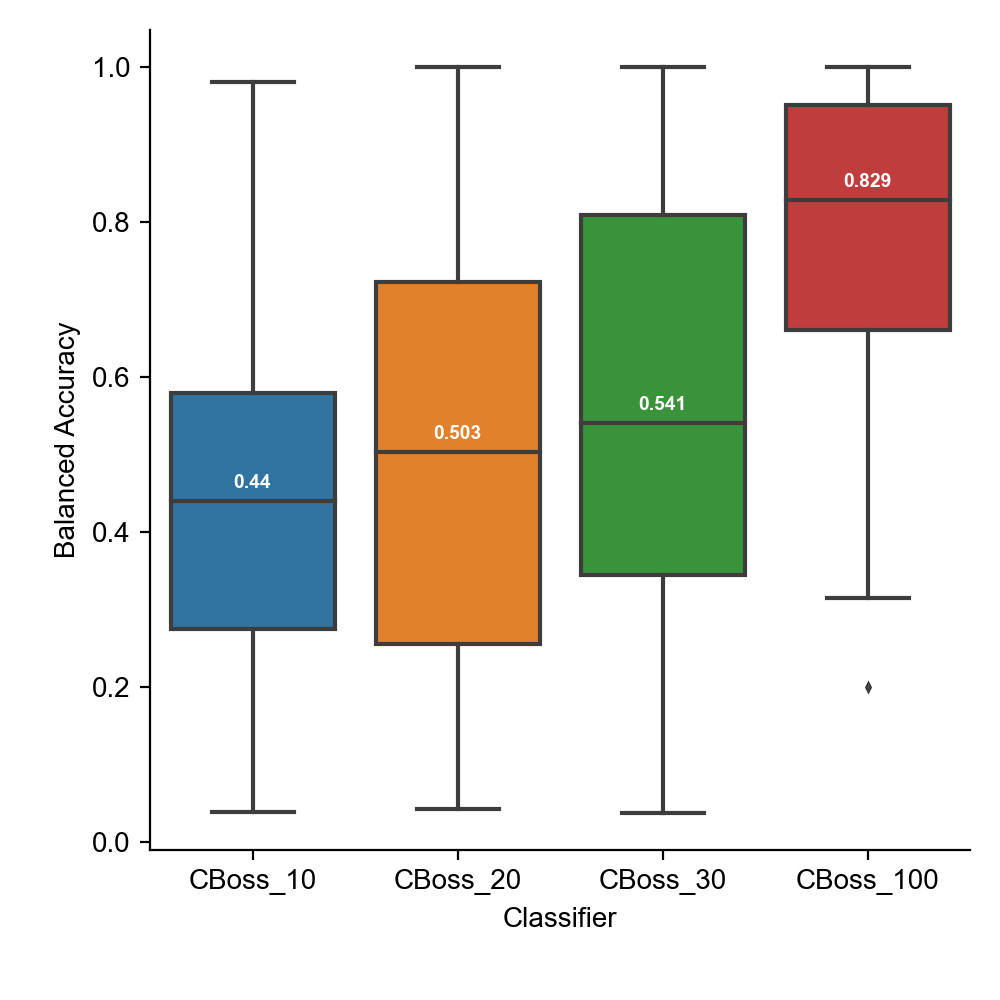
\includegraphics[width=0.49\textwidth,keepaspectratio]{boxplot_accuracy_CBoss.png}
  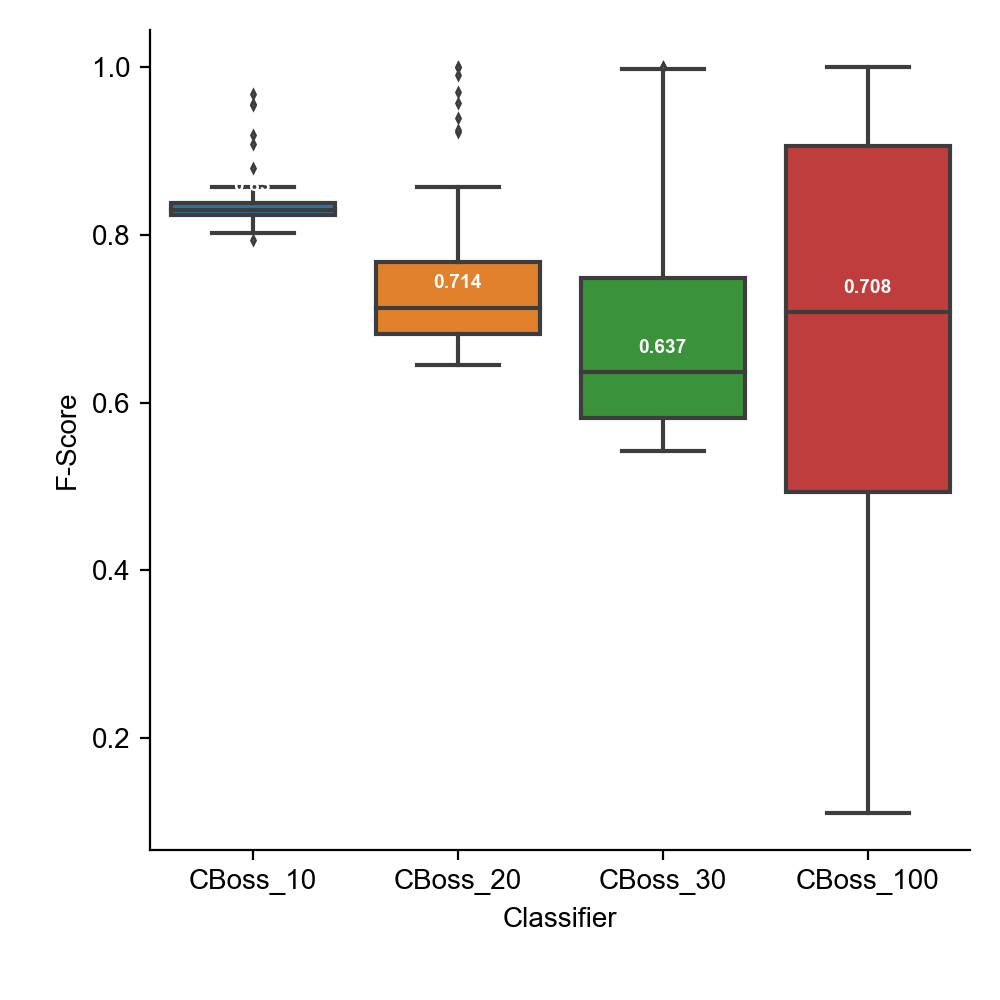
\includegraphics[width=0.49\textwidth,keepaspectratio]{boxplot_f_score_1_CBoss.png}
  \caption{Comparison between Balanced Accuracy (left) and $F_{1}$ (right) for CBoss}
  \label{fig:FBeta1}
\end{figure}

By checking the boxplots for the $F_{1}$, we find that the median value for the 10\% version is \textbf{0.83}, while the median value of the 100\% version is \textbf{0.708}.
Also the distribution of the values for the 10\% version is very close to the median and the minimum value is higher than the median of the 100\% version.
Which means that even for the data sets on which the 10\% version of CBoss scores very low accuracy scores, it will still get a high $F_{1}$ relative to the 100\% version.
The harmonic mean over-compensates for the lower accuracy scores with very high values for earliness causing misleading values.

To decide which $\beta$ value is best to use, we carried out a sequence of experiments using $\beta$ = [0.1, 0.9].
The value that gave the most reasonable results was 0.5.
Figure \ref{fig:FBeta05} shows the same comparison between the boxplots of $Balanced Accuracy$ and $F_{\beta}-measure$ for CBoss but with $\beta$ = 0.5.
Still $F_{1}$ allows for compensation between accuracy and earliness for the 10\% version, but it refines the values.
The median value for the 10\% version became \textbf{0.705} while that of the 100\% is \textbf{0.795}.
The distribution of values for the 10\% is spread more and the maximum value is falling near the median value of the 100\%.

\begin{figure}[!htbp]
  \captionsetup{justification=raggedright}
  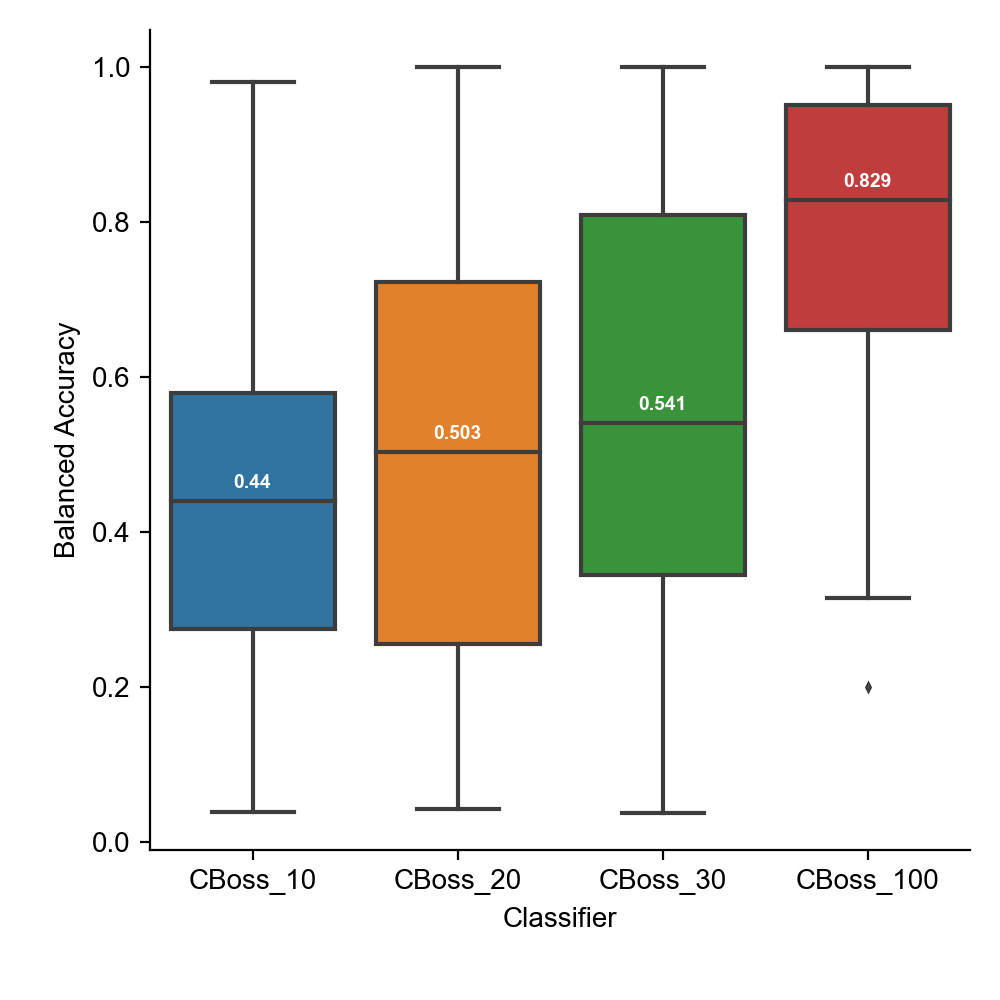
\includegraphics[width=0.49\textwidth,keepaspectratio]{boxplot_accuracy_CBoss.png}
  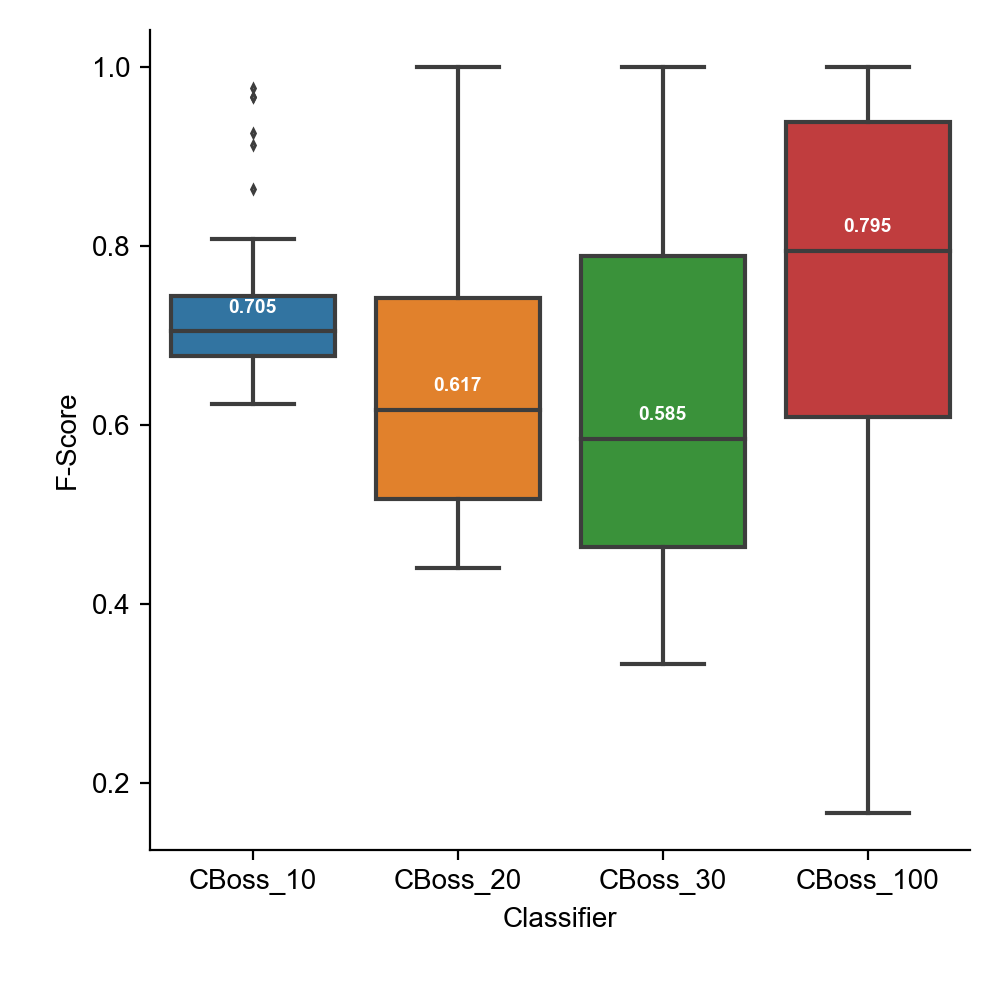
\includegraphics[width=0.49\textwidth,keepaspectratio]{boxplot_f_score_05_CBoss.png}
  \caption{Comparison between Balanced Accuracy (left) and $F_{0.5}$ (right) for CBoss}
  \label{fig:FBeta05}
\end{figure}

We believe that selecting the best value of $\beta$ is not trivial.
It is problem dependant and not one specific value can fit for all problems.
For our experiments we decided to give earliness less priority than performance,
but in other situations it might be the case that both of them contribute with the same importance or even earliness is more critical.


\subsection{The Recommender Experimental Design}
\label{SubsectionRecommenderExperiment}
As previously discussed in the recommender design, we train one random forest regressor per chunk, which we call the chunk learner.
Each chunk learner is trained on the results for a specific chunk and is responsible for predicting the performance score, $F_{\beta}-measure$, for all classifiers on unseen data sets for that specific chunk.

% data sets used
To train the chunk learners, we use the results of experiments from the testbed combined with metadata about the data set.
Each training instance consists of metadata features from the table \ref{tab:long} in addition to 3 features from the testbed results in table \ref{TableAnalysisReport}; the classifier name, the revealed\% and the $F_{\beta}-measure$ value.
The results of all data sets are included in the learning process, regardless of whether they were finished by all the classifiers and for all the chunks or not.
We only exclude the three data sets PEMS-SF, DuckDuckGeese and FaceDetection; because they were only finished by one classifier. Which leaves us with 74 data sets.

%  Overall description
In the beginning, we randomly split the data into training and testing data sets.
Then for each chunk learner, we start a grid search process, on the training data, for learning hyperparameters and model selection.
In the end, the chunk learners are evaluated using the best selected model on the unseen testing data sets for the final evaluation.

% detailed description of training and testing
For the creation of training and testing data sets, we use an 80/20 split with random selection.
A total of 59 data sets are used for the learning of chunk learners, while 15 data sets are left out for the final evaluation.

For the training of the chunk learners we use a grid search; to select the best combination of hyperparameters for each chunk learner model for its designated chunk.
During the grid search operation, a 10-fold cross validation process is carried out in which each training model is trained and evaluated 10 times.
The final score for each model is represented by its average across all 10-folds.
We define the hyperparameter space for 2 parameters of the random forests; the maximum depth of trees = \{3, 5, 10, $\infty$\} and the number of trees per forest = \{2, 3, 4, 5, 10, 50, 100, 250, 500\}.
After the grid search is finished, the best performing model is selected to be used as the final chunk learner on the unseen testing data sets.
To avoid biases in the results of the chunk learners from the selection of training and testing data sets, this whole process is repeated 50 times using random selection of the data sets for training and testing.
We use the seeds = [0, 49] for the random selection of data sets and for the bootstrapping and sampling of features in the building for trees; to allow for reproducability of the results.

% preprocessing (one hot encoding)
Since we are using regression random forests, one mandatory preprocessing step has to be carried out; to transform the cateogrical features into numerical features.
We do \emph{one-hot-encoding} on the the two features $classifier$ and $type$, which represent the name of the classifier that was used and the type of the data set respectively.

